\documentclass[a4paper, 11pt]{article}
\usepackage[french]{babel}
\usepackage[utf8]{inputenc}
\usepackage[T1]{fontenc}
\usepackage{datetime}
\usepackage{float}
\usepackage{eurosym}
\usepackage{comment} % enables the use of multi-line comments (\ifx \fi)
\usepackage{graphicx}
\usepackage{eurosym}

\usepackage{framed, color} % shade-box around the text to highlight
\definecolor{shadecolor}{RGB}{211,211,211}

\usepackage{fullpage} % changes the margin

\begin{document}
%Header-Make sure you update this information!!!!
\noindent
\large\textbf{Cahier des charges} \hfill \textbf{Distribution de l'eau en Haïti} \\
\normalsize Deknop Céline \hfill Université catholique de Louvain \\
Hallet Adrien \hfill \today \\
Strebelle Sébastien

\section*{Abstract}
Cahier des charges du projet de gestion de distribution d'eau en Haïti, mémoire UCLouvain 2018-2019. Destiné aux intervenants du projet et contenant les propositions pour la future application.
\hrule
\section{Glossaire}
% Liste exhaustive de tous les termes pouvant prêter à confusion
  \begin{description} %ToDo : trouver un moyen de display ça beau, je sais pas si c'est l'idéal. Aussi y'a pas moyen d'auto-sort par ordre alphabétique ?
    %ToDo 2 : définir les termes
    %ToDo 3 : ordonner alphabétiquement le truc si on peut pas le faire automatiquement
    %ToDo 4 : check le document régulièrement et ajouter tous les termes qui peuvent prêter à confusion
    \item[CAEPA] Comité d'Approvisionnement en Eau Potable et d'Assainissement. Entité haïtienne chargée de toute activité nécessaire aux systèmes d'eau potable.
    \item[DINEPA] Direction Nationale de l'Eau Potable et de l'Assainissement. Entité haïtienne rattachée au gouvernement, chargée d'exécuter la politique étatique dans le secteur de l'eau et assainissement.
    \item[HTG] Devise (monnaie) d'Haïti, la \emph{Gourde} ($\approx 0,012$ \euro \footnote{Cours consulté le 03 octobre 2018})
    \item[Application ou système] Ensemble des productions relatives à l'outil informatique en cours de création pour la gestion de l'eau et facturation en Haïti.
    \item[Utilisateur] Un être humain interagissant avec l'application.
    \item[Interface (graphique)] Dispositif visuel permettant à l'utilisateur d'interagir avec l'application (\emph{i.e. : ce qui s'affiche à l'écran}).
    \item[Donnée] Information enregistrée dans l'application destinée à une ou plusieurs utilisations (\emph{e.g. : la quantité d'eau utilisée})
    \item[Permission (accès)] Droit informatique permettant à l'utilisateur d'accéder à des fonctionnalités ou données de l'application.
    \item[Accès en lecture] Droit informatique autorisant la consultation d'une information.
    \item[Accès en écriture] Droit informatique autorisant la modification d'une information (implique l'accès en lecture).
    \item[Éléments du réseau de distribution de type "sortie"] %TODO change in text
    \item[Profils]
    \item[Citizen science]
    \item[Scalable]
    \item[Réseau]
    \item[Fontaine]
    \item[Kiosque]
    \item[Réservoir]
    \item[Prise individuelle]
    \item[Zone (du réseau)]
    \item[Rapport mensuel]
    \item[Ticket]
  \end{description}
\section{Introduction}
% Contexte de l'application
Dans chaque section du document, nous avons ajouté une partie "Questions et remarques", où nous demandons à Protos ou aux intervenant Haïtiens de donner des précisions ou leur avis car nous estimons n'avoir pas assez d'informations ou de connaissances sur le sujet. Ce sont les points sur lesquels nous avons le plus besoin d'aide et dont il faut discuter en priorité, mais toute remarque sera prise en compte et appréciée.
\section{Types d'utilisateurs}
Cette section du document contient une description détaillée de tous les types d'utilisateurs qui, à terme, interagiront avec l'application. Nous détaillons aussi ce que ceux-ci pourront faire avec l'application, pour vous donner un contexte familier.

  \begin{description}
    \item[Gestionnaire de fontaines] est un utilisateur auquel on assigne un ou plusieurs éléments du réseau de distribution de type "sortie" (fontaine, kiosque, réservoir, branchement individuel) dont il est responsable.
    Il gère également la gestion des consommateurs d'eau dans sa zone et les ajoute/supprime/modifie dans le système lorsque c'est nécessaire (naissance, décès, déménagement).
    Il utilise l'application pour signaler des problèmes et ainsi pouvoir en avertir le technicien/plombier et sa hiérarchie. Chaque mois, le gestionnaire de fontaines utilise l'application pour déposer un rapport. Ce rapport contient, pour chaque élément du réseau sous sa responsabilité, les quantités d'eau distribuées (si un compteur est présent), les recettes (HTG), l'état (en service, hors service). Une section générale (une seule fois par rapport) déclare également les heures et jours de service du gestionnaire de fontaines.

    \emph{Exemple : une personne chargée de gérer un point d'eau pourrait être un gestionnaire de fontaine. Il peut ainsi utiliser l'application pour envoyer mensuellement les données, ajouter les utilisateurs lorsque nécessaire et déclarer les problèmes.}

    \item[Gestionnaire de zone] est un utilisateur qui gère un groupe de gestionnaires de fontaines. Il dispose des mêmes permissions que les gestionnaires de fontaines dans sa zone et peut donc effectuer les mêmes actions avec l'application. En plus de ça, le gestionnaire de zone peut créer des profils de gestionnaires de fontaines et de techniciens/plombiers et leur assigner des permissions sur les éléments du réseau. %Meh

    \emph{Exemple 1 : Protos ou la DINEPA peuvent être assignés en tant que gestionnaires de zone ayant les accès sur tous les systèmes et agir en tant que gestionnaires généraux de tout le système. Ils peuvent donc consulter toutes les informations rapportées par les autres utilisateurs.}

    \emph{Exemple 2 : un CAEPA pourrait être assigné en tant que gestionnaire de zone et avoir accès aux infrastructures du réseau de distribution dans sa zone géographique et ainsi consulter les informations et les modifier pour venir en aide aux gestionnaires de fontaine.}

    \item[Consommateur] est un utilisateur du réseau de distribution d'eau, mais dans un premier temps, n'aura pas accès à l'application. Dans le futur, une nouvelle fonctionnalité de l'application lui permettra de signaler un problème sur le réseau, de consulter l'état de celui-ci et éventuellement d'autres fonctionnalités, qui seront détaillées par la suite.

    \item[Technicien/Plombier] est un utilisateur auquel on assigne des éléments du réseau de distribution (fontaine, réservoir, prise individuelle, etc). Chaque technicien/plombier utilise l'application pour voir les problèmes déclarés par les autres utilisateurs (gestionnaires de fontaine, de zone ou consommateurs quand le volet \emph{Citizen science} sera ajouté). Il peut utiliser l'application pour répondre aux demandes d'intervention pour demander plus d'informations ou proposer une solution si le déplacement n'est pas nécessaire. Il peut modifier l'état d'un problème, demander des précisions et le marquer en cours de résolution ou résolu une fois l'intervention terminée.

    \emph{Exemple : un technicien plombier démarrant sa journée peut consulter l'application et voir quels sont les problèmes qui requièrent son attention. Il peut dialoguer avec les gestionnaires et modifier l'état des problèmes afin qu'à terme le réseau fonctionne sans problème.}

  \end{description}
  \subsection{Questions et remarques}
  % Questions
  \begin{itemize}
    \item Le contenu du rapport mensuel d'un gestionaire de fontaine sera un élément essentiel de l'application. S'il manque quoique ce soit, précisez-le nous au plus vite.
    \item Un gestionnaire de zone dont la zone recouvre tous les systèmes peut être vu comme un administrateur et aurait dès lors accès en lecture et écriture à toutes les données de l'application. Par erreur ou malveillance, il pourrait en effacer ou modifier certaines, faussant l'ensemble. Une pratique courante en informatique pour gérer ce problème potentiel est d'archiver les données : elles ne sont ainsi jamais vraiment modifiées ou effacées et peuvent être restaurées à l'état précédent. Est-ce une fonctionnalité que vous souhaitez pour l'application, ou n'est-ce pas nécéssaire de s'en occuper ? Si ce modèle d'archivage ne vous convient pas, souhaitez-vous autre chose ?
    \item L'utilisateur "technicien/plombier" et les fonctionnalités qui lui seront associées sont une interprétation de notre part car il nous semblait pratique de pouvoir centraliser la gestion du réseau de distribution entièrement au sein de l'application. Cela vous semble-t-il utile d'avoir une interface destinée au technicien ?
  \end{itemize}

\section{Fonctionnalités}
% Liste exhaustive des fonctionnalités de l'application
% Séparer directement en fonction des différents utilisateurs de l'application

  \subsection{Questions et remarques}
\section{Exemples}
  \begin{shaded}
    Les visuels d'écran présents dans cette section sont des schémas. Ils cherchent à donner une idée de ce à quoi ressemblera l'application en terme de contenu. Les couleurs, agencements et formes ne représentent en rien l'esthétique finale de l'application. Vos désirs esthétiques sont en revanche bienvenus si vous avez des idées ou souhaits.
  \end{shaded}

  \subsection{Accueil}

    \begin{figure}[H]
        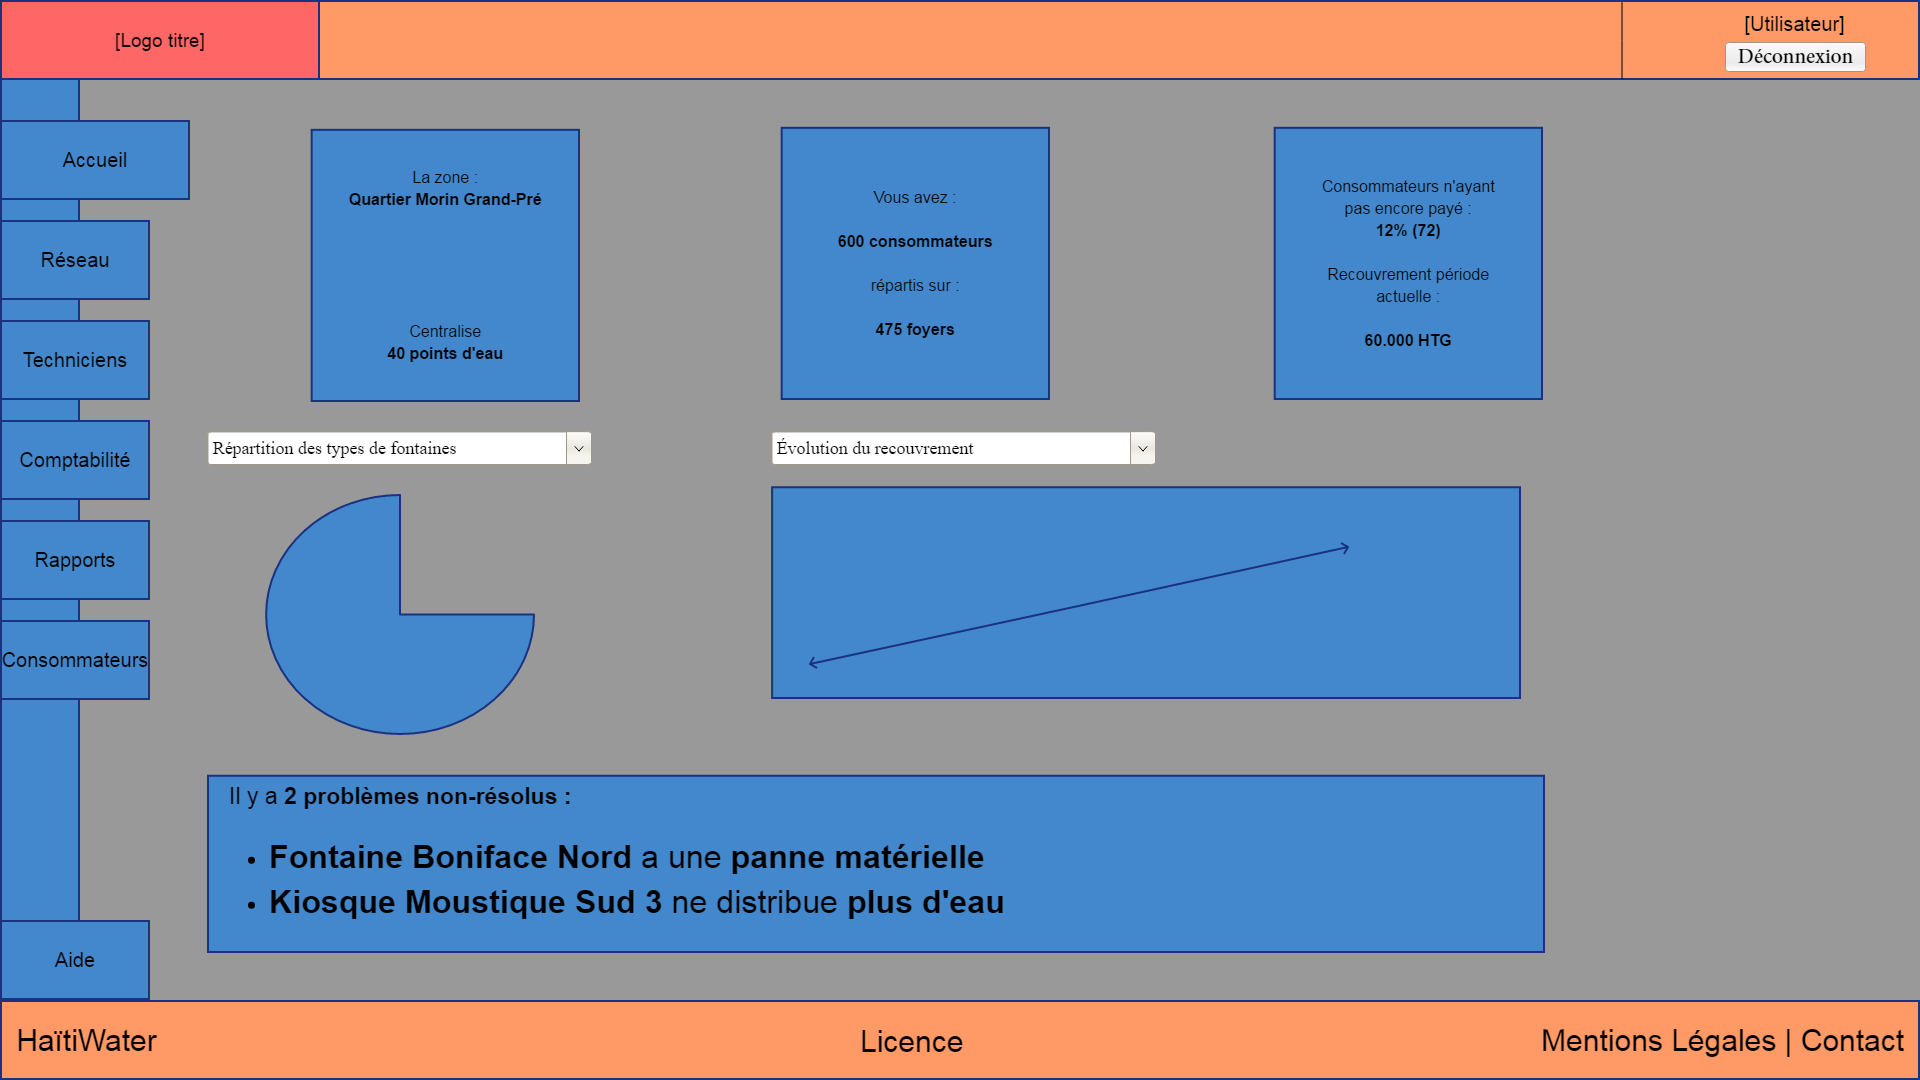
\includegraphics[width=\textwidth]{Cahier_des_Charges/accueil}
        \caption{\'Ecran d'identification}
        \label{fig:zone_dashboard}
    \end{figure}

    Une fois identifié par son nom d'utilisateur et mot de passe, l'utilisateur arrive sur son tableau de bord. Le tableau de bord est personnalisé pour chaque catégorie d'utilisateur (gestionnaire de zone, de fontaine, technicien/plombien).

    La figure~\ref{fig:zone_dashboard} présente le tableau de bord du gestionnaire de zone. En en-tête, l'utilisateur peut cliquer sur le logo de l'application pour retourner à ce même tableau de bord à tout moment de sa navigation. Il peut aussi se déconnecter.

    \'A gauche, le menu principal indique à l'utilisateur les pages auxquelles il peut accéder en cliquant sur les boutons. Le bouton étendu indique à l'utilisateur sur quelle page il se trouve (ici "Accueil").

    Au centre, le contenu de la page propose tout d'abord trois zones informatives générales :
    \begin{itemize}
      \item Zone courante, son nom et le nombre de points d'eau (kiosques, fontaines, réservoirs, prises individuelles)
      \item Consommateurs, total, nombre de foyers
      \item Recettes, pourcentage de recouvrement des paiements, recettes totales
    \end{itemize}
    L'utilisateur peut cliquer sur chacune des zones pour aller sur la page comprenant le détail des informations (respectivement les pages \emph{Réseau, Consommateurs, Comptabilité})

    Ensuite, des graphiques sont proposés à l'utilisateur (ici, la répartition des types de points d'eau et l'évolution du taux de recouvrement en fonction du temps). L'utilisateur peut uiliser la flèche à droite du titre du graphique pour en choisir un autre (quantité d'eau distribuée en fonction du mois, évolution du nombre de consommateurs, ...).

    Enfin, une zone de notification alerte l'utilisateur des problèmes non-résolus sur le réseau de distribution d'eau. Il peut également cliquer dessus pour aller à la page des problèmes.

  \subsection{Rapports et problèmes}
    \begin{figure}[H]
        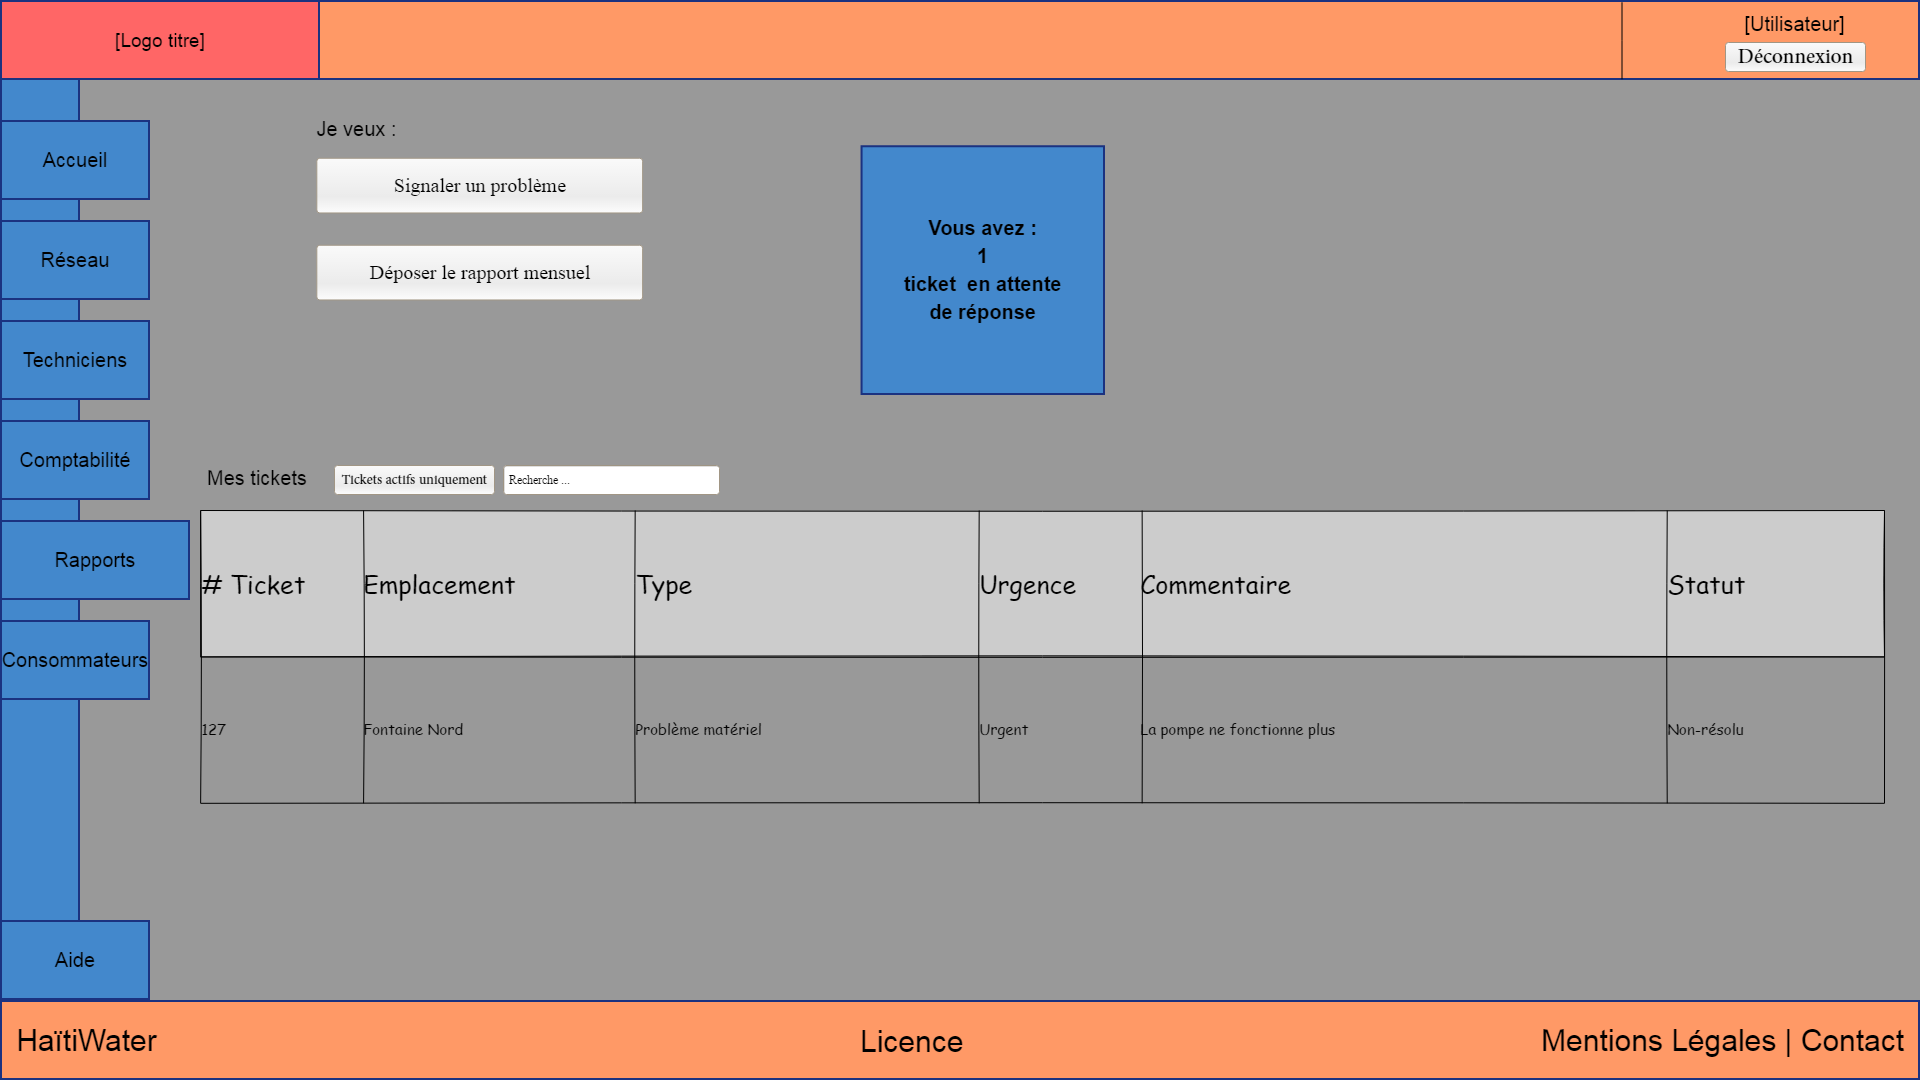
\includegraphics[width=\textwidth]{Cahier_des_Charges/rapports}
        \caption{\'Ecran des rapports}
        \label{fig:report}
    \end{figure}
    La figure~\ref{fig:report} présente la vue de rapport d'un gestionnaire de zone et d'un gestionnaire de fontaines. Le gestionnaire peut signaler un problème ou déposer le rapport mensuel (voir figure~\ref{fig:monthly_report}).

    En dessous, le gestionnaire voit la liste de ses tickets en cours de traitement et leur statut. En cliquant dessus, il peut répondre aux messages du technicien (qui peut lui demander des précisions, proposer une solution, ...). Des notifications alertent le gestionnaire lorsqu'il a reçu une réponse à son ticket.

    \begin{figure}[H]
        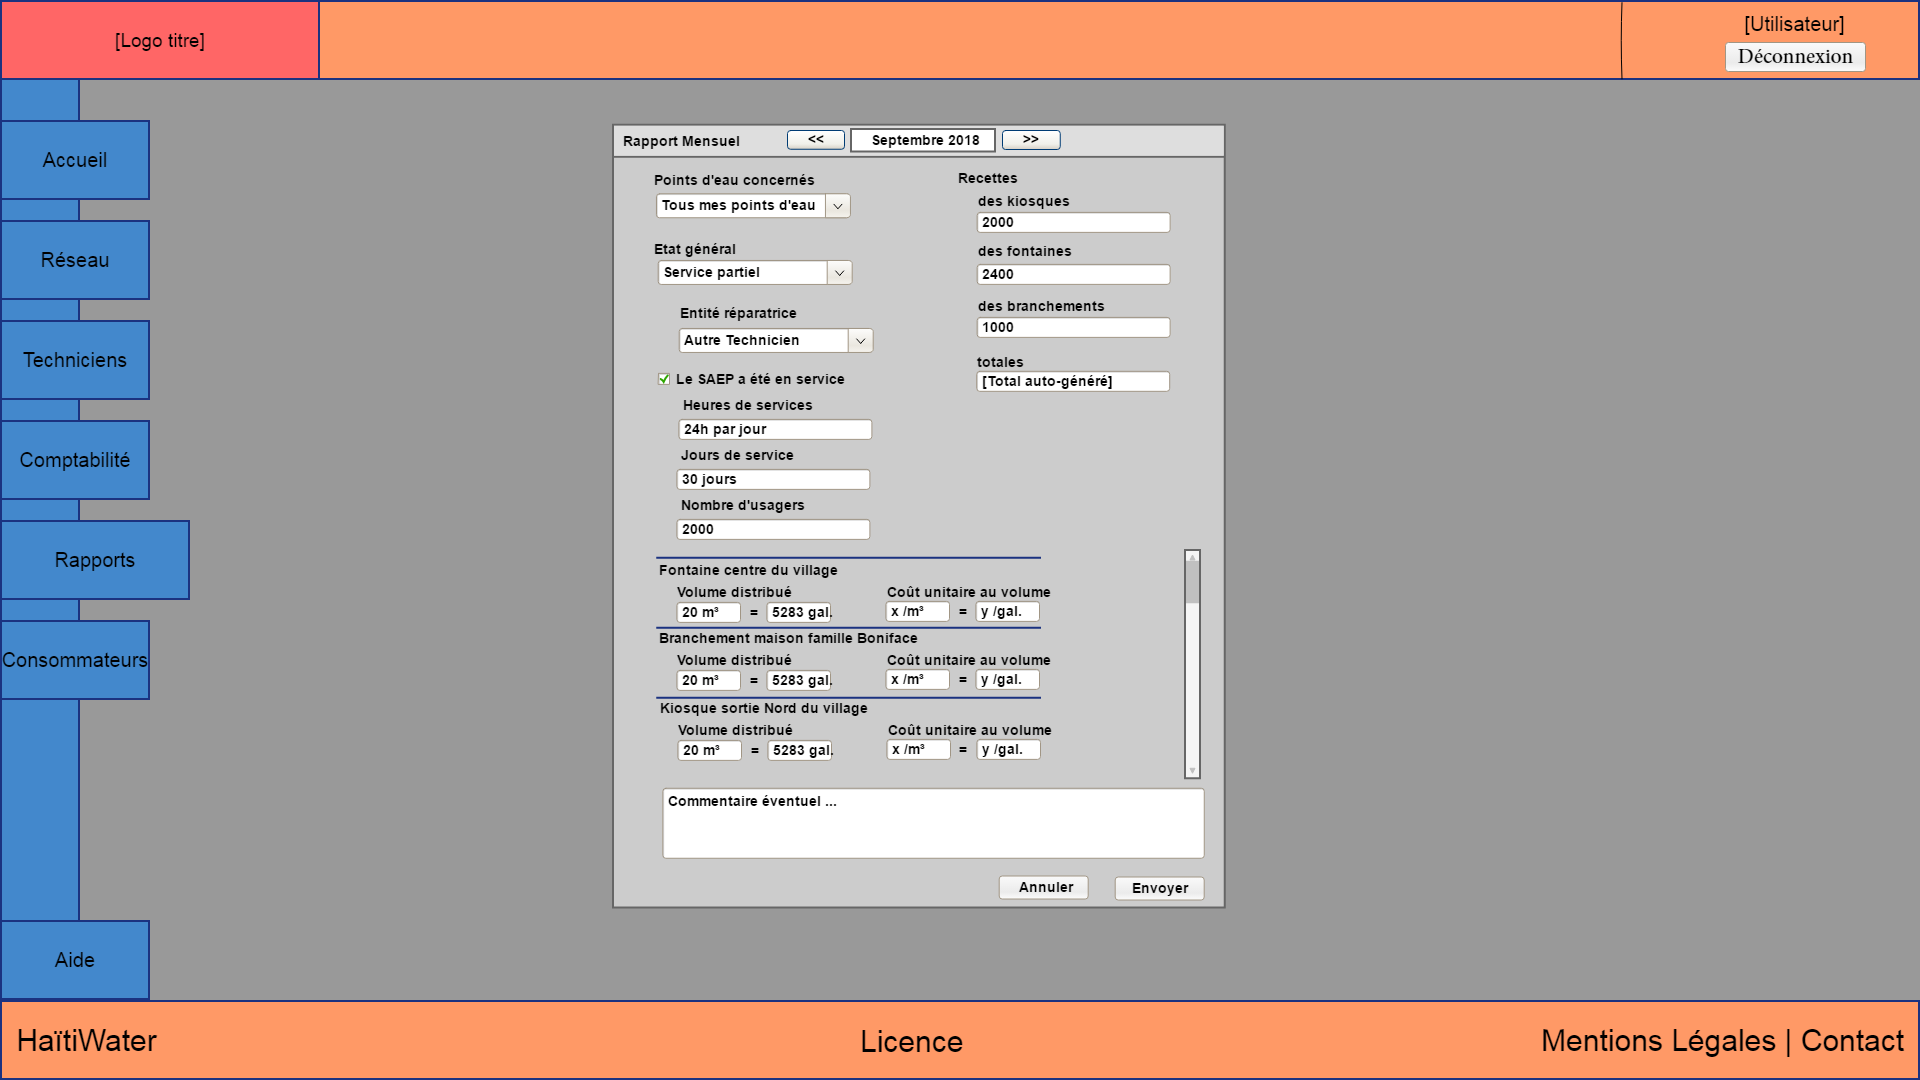
\includegraphics[width=\textwidth]{Cahier_des_Charges/rapports_mensuel}
        \caption{Rapport mensuel}
        \label{fig:monthly_report}
    \end{figure}

    En figure~\ref{fig:monthly_report}, le gestionnaire fait son rapport mensuel. Chaque mois, ce formulaire doit être rempli pour obtenir les données du réseau. Si un rapport a déjà été rempli (par exemple si le gestionnaire de zone accède au rapport mensuel et qu'une partie des données a déjà été remplie par un gestionnaire de fontaines), il peut être modifié par ce même moyen.

    Ici, nous voyons le formulaire d'un gestionnaire de fontaines. Il se présente en cinq parties ;
    \begin{itemize}
      \item Le gestionnaire de fontaines sélectionne la ou les sorties d'eau (fontaine, prises individuelles, kiosques, réservoirs) qui lui sont attribuées et pour lesquelles il souhaite faire son rapport.
      \item Le gestionnaire de fontaines indique s'il a pu être en service durant ce mois, si oui il indique le nombre de jours et d'heures durant lesquels le service était disponible.
      \item Le gestionnaire de fontaines indique les recettes pour les fontaines, kiosques et branchements individuels, le total est affiché automatiquement.
      \item Pour chaque sortie d'eau sélectionnée au début du rapport, le gestionnaire de fontaines indique la quantité d'eau distribuée ainsi que les prix de distribution.
      \item Le gestionnaire de fontaines peut enfin ajouter un commentaire au rapport mensuel.
    \end{itemize}

    Le gestionnaire peut soumettre le rapport quand il le souhaite, même partiellement complété. Il peut y revenir plus tard et modifier les informations.

  \subsection{Vue du réseau}
    \begin{figure}[H]
        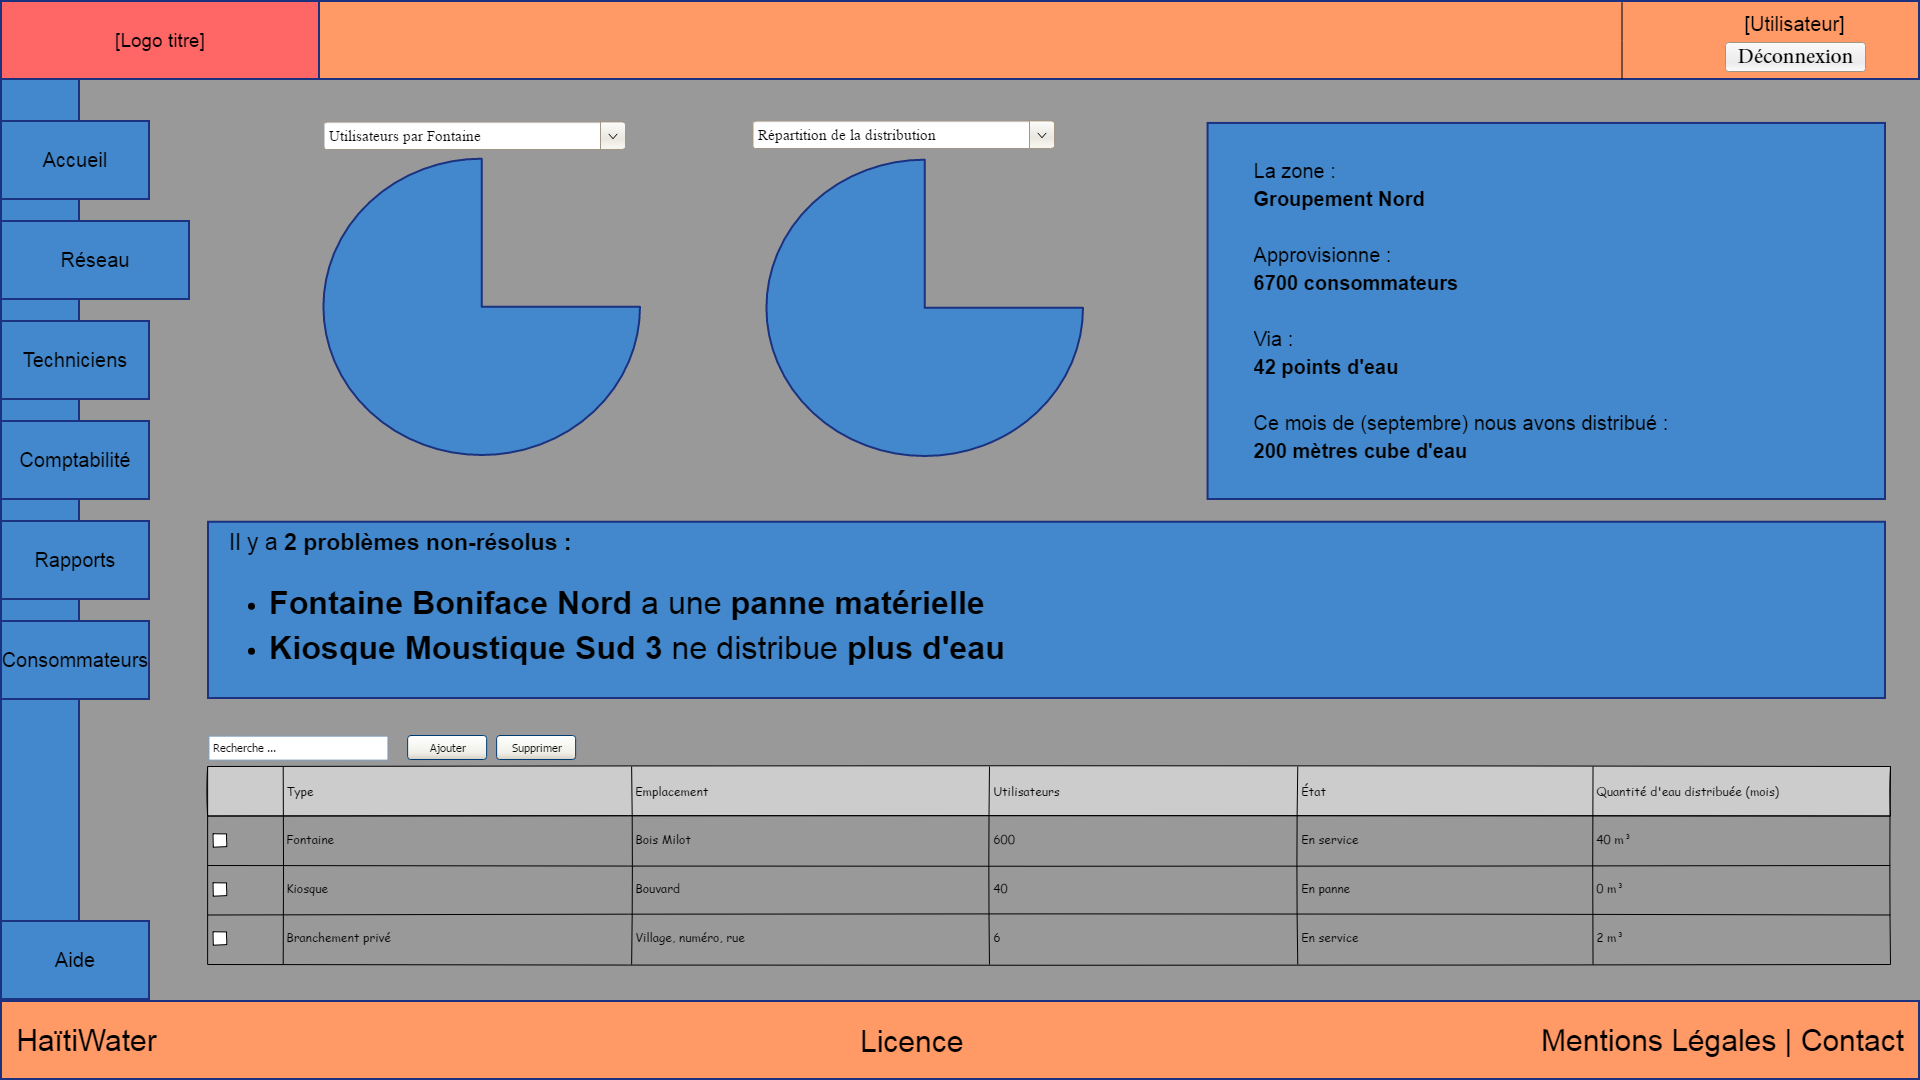
\includegraphics[width=\textwidth]{Cahier_des_Charges/reseau}
        \caption{Visuel du réseau}
        \label{fig:network}
    \end{figure}
    La figure~\ref{fig:network} présente la vue d'accueil du réseau de distribution. A partir de cette page, le gestionnaire de distribution ou de fontaines peut voir les installations du réseau qui lui sont attribuées. Il y a à nouveau un espace dédié aux graphiques qu'il peut choisir et visualiser via la flèche à droite du titre.

    A droite, des informations générales sont disponibles ainsi que des statistiques (ici, le volume mensuel total distribué en exemple).
    L'utilisateur voit à nouveau un écran de notifications indiquant les problèmes qu'il faut résoudre.

\section{Besoins non-fonctionnels}
Dans cette section, nous allons détailler certaines caractéristiques souhaitables pour l'application. Il s'agit d'exigences sur le système en lui-même et pas sur ce qu'il fait.
\begin{enumerate}
  \item Système performant pour permettre une utilisation dans les conditions haïtiennes.
  \item Sécurité des données.
  \item Fonctionnement sur périphérique mobile (tablettes et smartphones).
  \item Présence d'une documentation qualitative pour les développeurs et les utilisateurs du système.
  \item Application scalable pour permettre une utilisation à différentes échelles.
\end{enumerate}
% Explication des besoins non-fonctionnels
\section{Approche}
  Pour créer ce cahier des charges qui établit les fonctionnalités et le fonctionnement général de l'application, nous avons utilisé les documents fournis par Protos et disponibles en ligne
  \begin{description}
    \item[Les fichiers Excel], au nombre de trois ont été principalement utilisés pour le choix des données et fonctionnalités de l'application. Deux des fichiers concernent les CAEPA et recensent leurs fontaines, consommateurs et comptabilités à l'échelle annuelle. Un fichier expose au niveau national et mensuel l'état du réseau (fonctionnement, quantités d'eau distribuées) et les recettes envoyées via formulaire par des TEPAC qui gèrent le réseau à leur échelle sur le terrain.
    \item[Les documents de contexte] envoyés par Protos faisant état de la situation en Haïti, le projet de Protos sur place et leur fonctionnement.
    \item[Le rapport de capitalisation] fourni récemment et expliquant le processus, pour Poste Métier, de fonctionnement de la distribution de l'eau.
  \end{description}
  Les fichiers Excels ont été notre plus grande source d'information puisqu'ils nous permettent de connaître le système informatique actuel, quelles sont les données, comment sont-elles collectées et utilisées.
  Les fichiers de contexte ont permis de comprendre la situation, d'identifier les intervenants et risques de l'application.
  Le rapport de Poste Métier a été très intéressant pour comprendre le fonctionnement précis d'une zone du réseau de distribution.

  Notre approche générale dans cette application est d'automatiser la collecte et faciliter la gestion de toutes les données présentes dans les documents Excel actuellement utilisés en Haïti. Dans ce cahier des charges, nous présentons une application hiérarchique où chaque utilisateur fait remonter l'information dont il dispose (exactement comme le fonctionnement actuel des données Excel qui sont extraites des formulaires).

  \begin{shaded}
    Si ce cahier des charges vous semble incorrect (incompréhension d'une fonctionnalité) ou incomplet (manque de fonctionnalités), tout nouveau document permettant de mieux comprendre votre fonctionnement et vos désirs pour l'application est le bienvenu.
  \end{shaded}

\section{Choix technolgiques}
  Conformément aux demandes, l'application utilisera des technologies gratuites. Les décisions des technologies utilisées dans le développement tentent de maximiser :
  \begin{description}
    \item[Popularité] Plus une technologie est populaire, plus elle est susceptible d'être maintenue à jour, de disposer de guides et d'aides en ligne.
    \item[Simplicité] Pour permettre aux futurs développeurs de l'application de la maintenir à jour et de la faire évoluer avec un minimum de connaissances requises.
    \item[Performance] Afin que l'application soit utilisée le plus longtemps possible et qu'il ne soit pas nécessaire de recommencer à zéro à cause d'une technologie limitant l'application.
  \end{description}

  Sur ces bases, nous avons déjà arrêté les choix généraux suivants.
  \begin{description}
    \item[Interface] Les langages HTML5, CSS3 et JavaScript sont les plus populaires et peu d'alternatives existent pour le développement d'applications internet, aucune n'étant aussi simple à utiliser.
    \item[Application] Nous allons utiliser le framework\footnote{Framework : structure logicielle encadrant l'application, permettant d'automatiser certaines phases du développement} Django, le sixième plus populaire avec un score de 94\%\footnote{statistique de https://hotframeworks.com/, septembre 2018} et qui permet de programmer la logique de l'application dans le langage Python, très populaire et adapté autant pour un débutant que pour un expert en programmation.
    \item[Base de Données] Pour stocker les données, nous allons utiliser la technologie SQL avec le système de gestion PostgreSQL\footnote{Quatrième mondial selon https://db-engines.com/en/ranking} qui présente l'énorme avantage d'avoir un module géographique (PostGIS) qui peut interagir directement avec le module géographique de l'application (GeoDjango).
  \end{description}
\end{document}
